\documentclass{statsoc}
\usepackage[a4paper]{geometry}

\usepackage{natbib, dsfont, enumitem,
  amssymb,soul,xcolor,amsmath,graphicx,verbatim,pgfplots,tikz,prodint,booktabs}

%% Theorem environment
% \theoremstyle{plain} % plain italic style
\newtheorem{theorem}{Theorem}
\numberwithin{theorem}{section}
\newtheorem{lemma}[theorem]{Lemma}
\newtheorem{proposition}[theorem]{Proposition}
\newtheorem{corollary}[theorem]{Corollary}

%% Only for comments:
\usepackage[author=]{fixme}
\fxusetheme{color}
\definecolor{fxtarget}{rgb}{.5,.5,.5}
\definecolor{fxnote}{rgb}{.5,.5,.5}
\fxsetup{status=draft}

\bibliographystyle{rss}

% New operators and commands
\DeclareMathOperator{\E}{\mathbb{E}} % expectation
\newcommand{\Z}{\mathbb{Z}}
\newcommand{\R}{\mathbb{R}}
\newcommand{\N}{\mathbb{N}}
\newcommand{\C}{\mathbb{C}}
\renewcommand{\S}{\mathbb{S}}
\newcommand{\blank}{\makebox[1ex]{\textbf{$\cdot$}}}
\newcommand\independent{\protect\mathpalette{\protect\independenT}{\perp}}
\def\independenT#1#2{\mathrel{\rlap{$#1#2$}\mkern2mu{#1#2}}}
\renewcommand{\phi}{\varphi}
\renewcommand{\epsilon}{\varepsilon}
\newcommand*\diff{\mathop{}\!\mathrm{d}}
\newcommand{\weakly}{\rightsquigarrow}
\newcommand\smallO{\textit{o}}
\newcommand\bigO{\textit{O}}
\newcommand{\midd}{\; \middle|\;}
\newcommand{\1}{\mathds{1}}
\usepackage{ifthen} %% Empirical process with default argument
% \newcommand{\G}[1][]{%
%    \ifthenelse{ \equal{#1}{} }
%       {\ensuremath{\mathbb{G}_n}}
%       {\ensuremath{\mathbb{G}_{#1}}}
% }
% New version:
\newcommand{\G}[2][n]{
{\ensuremath{\mathbb{G}_{#1}}{\left[#2\right]}}
}
\DeclareMathOperator*{\argmin}{\arg\!\min}
\DeclareMathOperator*{\argmax}{\arg\!\max}
\newcommand{\empmeas}{\ensuremath{\mathbb{P}_n}} % empirical measure

\newcommand{\data}{\ensuremath{\mathcal{D}}}

\title[The state learner]{The state learner \\ {-- a super learner for right-censored data}}
\author[Anders Munch {\it et al.}]{Anders Munch}
\address{Section of Biostatistics, University of Copenhagen, Copenhagen, Denmark}
\email{a.munch@sund.ku.dk}
\author{Thomas A.\ Gerds}
\address{Section of Biostatistics, University of Copenhagen, Copenhagen, Denmark}


\begin{document}

\begin{abstract}
  In survival analysis, prediction models are needed as stand-alone tools and in
  applications of causal inference to estimate nuisance parameters. The super
  learner is a machine learning algorithm which combines a library of prediction
  models into a meta learner based on cross-validated loss. Unfortunately, the
  commonly used partial likelihood loss is not suited for super learning, and
  inverse probability of censoring weighted loss functions require a
  pre-specified estimator of the censoring distribution. To relax this, we
  introduce the state learner, a new super learner for survival analysis, which
  evaluates the loss based on the observed data simultaneously using libraries
  of predictions models for the event(s) of interest and the censoring
  distribution. We establish an oracle inequality for the state learner and
  investigate its performance through numerical experiments. We illustrate how
  the state learner allows us to estimate causal effects in a competing risks
  setting without having to pre-specify models for neither the cause-specific
  hazards of interest nor the censoring distribution.
\end{abstract}

\keywords{Loss based estimation, right-censored data, competing risks, super
  learner, cross-validation}

\section{Introduction}
\label{sec:introduction}

A super learner is a machine learning algorithm that combines a finite
set of learners into a meta learner by estimating prediction
performance in hold-out samples using a pre-specified loss function
\citep{van2007super}. When the aim is to make a prediction model,
super learners typically combine strong learners, such as Cox
regression models and random survival forests
\citep{gerds2021medical}.
% For targeted learning of a low dimensional
% target parameter in presence of a high-dimensional nuisance parameter,
% a super learner will usually also include the highly adaptive lasso
% \citep{van2011targeted, benkeser2016highly,van2017generally}.
While the general idea of combining strong learners based on cross-validation
data stems from earlier work \citep{wolpert1992stacked,breiman1996stacked}, the
name super learner is justified by an oracle inequality
\citep{van2003unicv,vaart2006oracle}: The super learner is guaranteed to perform
almost as well as the model which minimizes the expected performance, i.e., the
model we would select if we could evaluate the prediction performance in an
infinite hold-out sample.

We are concerned with the choice of the loss function for super learning in
survival analysis. Existing super learner algorithms for right-censored data use
partial log-likelihood loss or inverse probability of censoring weighted loss
\citep{polley2011-sl-cens,keles2004asymptotically,golmakani2020super,westling2021inference}.
The use of the partial log-likelihood loss restricts the class of learners and
excludes for example simple Kaplan-Meier based learners and also more complex
random survival forest algorithms. For this reason \cite{golmakani2020super}
restrict their learners to Cox proportional hazard models. A lesser known fact
is that a super learner constructed with the negative partial log-likelihood
loss implicitly depends on the censoring distribution
\citep{hjort1992inference,whitney2019comment}. A disadvantage of inverse
probability of censoring weighted loss functions is that they requires a
pre-specified model for the censoring distribution. \cite{westling2021inference}
tackle this challenge by iterating between super learning of the censoring
distribution and the event time distribution.

In this article we define the state learner, a new super learner for
right-censored data, which simultaneously evaluates the loss for learners of the
event time distribution and the censoring distribution. The loss function which
is used to define the state learner is only based on observable
quantities. The state learner can be applied to all types of survival
estimators, works in the presence of competing risks, and does not require a
single pre-specified estimator of the conditional censoring distribution. To
analyze the theoretical properties of the state learner we focus on the
so-called discrete super learner which `combines' the library of
learners by picking the one that minimizes the cross-validated loss. The state
learner uses separate libraries to model each competing event and the censoring
distribution. We show that the oracle selector of the state learner is
consistent if all libraries contain a consistent learner and prove a finite
sample oracle inequality.

The state learner can be used to select a model which predicts the probability
of an event based on covariates in the presence of competing risks. Another
application is in targeted learning where conditional event probabilities occur
as high-dimensional nuisance parameters which need to be estimated at a certain
rate \citep{van2011targeted, rytgaard2021estimation, rytgaard2022targeted}. We
show how a targeted estimator can be obtained from the state learner, and that a
second order product structure for the asymptotic bias term of the targeted
estimator is retained when the state learner is used to estimate nuisance
parameters.

The article is organized as follows. We introduce our notation and framework in
Section~\ref{sec:framework}. In Section~\ref{sec:super-learning} we define super
learning in general with right-censored data, and in
Section~\ref{sec:relat-liter-exist} we review existing methods.
Section~\ref{sec:super-learner-simple} introduces our novel proposal, the state
learner, and Section~\ref{sec:theor-results-prop} provides theoretical
guarantees for the state learner. In Section~\ref{sec:targeted-learning} we
discuss the use of the state learner in the context of targeted learning. We
report some numerical experiments in Section~\ref{sec:numer-exper} and analyze a
prostate cancer data set in Section~\ref{sec:real-data-appl}.
Section~\ref{sec:discussion} contains a discussion of the merits and limitations
of our proposal. Appendices~\ref{sec:proof-proposition}
and~\ref{sec:state-learner-with} contain proofs.


\section{Notation and framework}
\label{sec:framework}

In a competing risk framework \citep{andersen2012statistical}, let \( T\) be a
time to event variable, \(D\in\{1,2\}\) the cause of the event, and
$X \in \mathcal{X}$ a vector of baseline covariates taking values in a bounded
subset \( \mathcal{X} \subset \R^p \), \( p\in\N \). Let $\tau< \infty$ be the
maximal length of follow-up. We use \( \mathcal{Q} \) to denote the collection
of all probability measures on \( [0,\tau] \times \{1,2\}\times \mathcal{X} \)
such that \( (T, D, X) \sim Q \) for some unknown \( Q \in \mathcal{Q} \). For
\(j\in\{1,2\}\), the cause-specific conditional cumulative hazard functions are
defined by
\( \Lambda_{j} \colon [0, \tau] \times \mathcal{X} \rightarrow \R_+ \) such that
\begin{equation*}
  % \label{eq:cum-haz}
  \Lambda_{j}(t \mid x) = \int_0^t\frac{  Q(T \in \diff s, D=j \mid X=x )}{Q(T \geq s \mid X=x )}.
\end{equation*}
For ease of notation we assume throughout that \( \Lambda_j(\blank \mid x) \) is
continuous for all \( x \) and \( j \). We denote by \(S\) the conditional
event-free survival function,
\begin{equation}
  \label{eq:surv-def}
  S(t \mid x)=\exp\left\{-\Lambda_{1}(t \mid x)-\Lambda_{2}(t \mid x)\right\}.
\end{equation}
Let \( \mathcal{M} \) denote the space of all conditional cumulative hazard
functions on \( [0,\tau] \times\mathcal{X}\). Any distribution
\( Q \in \mathcal{Q} \) can be characterized by
\begin{equation*}
  \label{eq:parametrizeQ}
  \begin{split}
    Q(\diff t,j,\diff x)&= \left\{S(t- \mid x)\Lambda_1(\diff t \mid x)H(\diff x)\right\}^{1_{\{j=1\}}}\\
                        &\quad\left\{S(t- \mid x)\Lambda_2(\diff t \mid x)H(\diff x)\right\}^{1_{\{j=2\}}},
  \end{split}
\end{equation*}
where \(\Lambda_{j} \in \mathcal{M}\) for \(j=1,2\) and \(H\) is the marginal
distribution of the covariates.

We consider the usual right-censored setting in which we observe data
\(O = (\tilde{T},\tilde D, X)\), where $\tilde T = \min(T,C)$ for a
right-censoring time \(C\), $\Delta = \1{\{T \leq C\}}$, and
\(\tilde D=\Delta D\). Let \(\mathcal{P}\) denote a set of probability measures
on the sample space
\(\mathcal{O} = [0, \tau] \times \{0, 1, 2\} \times \mathcal{X}\) such that
\(O \sim P \) for some unknown \(P\in \mathcal{P}\). We assume that the event
time and the censoring time are conditionally independent given covariates,
\( T \independent C \mid X \). This implies that any distribution
\( P \in \mathcal{P} \) is characterized by a distribution
\( Q \in \mathcal{Q} \) and a conditional cumulative hazard function for \( C \)
given \( X \) \citep[c.f.,][]{begun1983information,gill1997coarsening}. We use
\(\Gamma\in\mathcal M\) to denote the conditional cumulative hazard function for
censoring. We assume that \( \Gamma(\blank \mid x) \) is continuous for all
\( x \), and let \(G(t \mid x)=\exp\left\{-\Gamma(t \mid x)\right\}\) denote the
survival function of the conditional censoring distribution. In our setting with
competing risks, this yields
\begin{equation}\label{eq:parametrizeP}
  \begin{split}
    P(\diff t, j, \diff x) &= \left\{G(t- \mid x)S(t- \mid x)\Lambda_1(\diff t \mid x)H(\diff x)\right\}^{\1{{\{j=1\}}}}\\
                           &\quad\left\{G(t- \mid x)S(t- \mid x)\Lambda_2(\diff t \mid x)H(\diff x)\right\}^{\1{{\{j=2\}}}}\\
                           &\quad\left\{G(t- \mid x)S(t- \mid x)\Gamma(\diff t \mid x)H(\diff x)\right\}^{\1{{\{j=0\}}}}\\
                           &=\left\{G(t- \mid x)Q(\diff t,j,\diff x)\right\}^{\1{{\{j\ne 0\}}}}\\    
                           &\quad\left\{G(t- \mid x)S(t- \mid x)\Gamma(\diff t \mid x)H(\diff x)\right\}^{\1{{\{j=0\}}}}.
  \end{split}
\end{equation}
Hence, we may write
\( \mathcal{P} = \{ P_{Q, \Gamma} : Q \in \mathcal{Q}, \Gamma \in
\mathcal{G} \} \) for some \( \mathcal{G} \subset \mathcal{M} \). We
also have
\begin{equation*}
P(\tilde T>t \mid X=x) = S(t \mid x)G(t \mid x) = \exp\left\{-\Lambda_{1}(t \mid x)-\Lambda_{2}(t \mid x)-\Gamma(t \mid x) \right\}.
\end{equation*}
We further assume that there exists \(\kappa<\infty\) such that
\(\Lambda_{j}(\tau- \mid x)<\kappa \), for \(j\in\{1,2\}\), and
\(\Gamma(\tau- \mid x)<\kappa\) for almost all \(x\in\mathcal X\). Note that this
implies that \(G(\tau- \mid x)\) is bounded away from zero for almost all \(x\in\mathcal X\).
Under these assumptions, the conditional cumulative hazard functions
\(\Lambda_{j}\) and \(\Gamma\) can be identified from \(P\) by
\begin{align}
  \Lambda_{j}(t \mid x) &= \int_0^t\frac{  P(\tilde T \in \diff s, \tilde D=j \mid X=x )}{P(\tilde T \geq s \mid X=x )}, \label{eq:lambdaj}\\
  \Gamma(t \mid x) &= \int_0^t\frac{  P(\tilde T \in \diff s, \tilde D=0 \mid X=x )}{P(\tilde T \geq s \mid X=x )}\label{eq:gamma}.
\end{align}
Thus, we can consider $\Lambda_j$ and \(\Gamma\) as operators which map from
\( \mathcal{P} \) to \(\mathcal M\).

 
\section{Super learning with right-censored survival data}
\label{sec:super-learning}

A super learner estimates a parameter $\Psi$ which can be identified from the
observed data distribution \(P\in\mathcal P\). In this section, to introduce the
concept of super learning, we simply consider estimation of the function
\( \Lambda_{j}\). The parameter \(\Psi:\mathcal P\to\mathcal M\) is then
identified via equation \eqref{eq:lambdaj} by \(\Psi(P)=\Lambda_j\).

As input to the super learner we need a sample \( \data_n=\{O_i\}_{i=1}^n \) of
i.i.d.\ observations from some unknown \( P \in \mathcal{P} \) and a finite
collection of candidate learners $\mathcal{A}$. Each learner
\(a \in \mathcal{A}\) is a map
\( a \colon \mathcal{O}^n \rightarrow \mathcal{M}\) which takes a data set as
input and returns an estimate $a(\data_n) \in \mathcal{M}$ of $\Lambda_{j}$.
% Formally, the domain of $a$ depends on \(n\) but we suppress this in the notation.
In what follows, we use the short-hand notation
\(P[f] = \int f(o) P(\diff o) \). A super learner evaluates the
performance of \(a \in \mathcal{A}\) using a loss function
\(L\colon \mathcal{M} \times \mathcal{O} \rightarrow \R_+\) by
estimating the expected loss \(P[L(a(\data_n), \blank)]\) using
cross-validation. Specifically, the expected loss of $a\in\mathcal A$
is estimated by splitting the data set $\data_n$ into $K$ disjoint
approximately equally sized subsets
\(\data_n^1, \data_n^2, \dots, \data_n^K \) and then calculating the
cross-validated loss
\begin{equation*}
  % \label{eq:cv-risk-est}
  \hat{R}_n(a; L) =
  \frac{1}{K}\sum_{k=1}^{K}
  % \empmeas^k{[L {(a{ (\data_n^{-k})} , \blank) }]},
  \frac{1}{| \data_n^{k} |}\sum_{O_i \in \data_n^{k}}
  L
  {
    \left(
      a{ (\data_n^{-k})}
      , O_i
    \right)
  },
  \quad \text{with} \quad
  \data_n^{-k} = \data_n \setminus \data_n^{k}.
\end{equation*}
% where \( \empmeas^{k} \) is the empirical measure of \( \data_n^{k} \). 
The subset \(\data_n^{-k}\) is referred to as the \(k\)'th training
sample, while \(\data_n^{k}\) is referred to as the \(k\)'th test or
hold-out sample.
The discrete super learner is defined as
\begin{equation*}
\hat{a}_n = \argmin_{a\in\mathcal A}\hat{R}_n(a; L).
\end{equation*}
The final estimator of \(\Psi(P)=\Lambda_j\) is then the selected
learner applied to the full data set, i.e., \(\hat{a}_n(\data_n)\).
The oracle learner is defined as the learner that minimizes the
average loss according to the data-generating distribution \( P \),
i.e.,
\begin{equation*}
  \tilde{a}_n =
  \argmin_{a \in \mathcal{A}}
  \tilde{R}_n(a; L),
  \quad \text{with} \quad 
  \tilde{R}_n(a; L)=
  \frac{1}{K}\sum_{k=1}^{K} 
  P{
    \left[
      L
      {
        \left(
          a{ (\data_n^{-k})}
          , \blank
        \right)
      }
    \right]}
  .
\end{equation*}
Note that both the discrete super learner and the oracle learner depend on the
library of learners and on the number of folds \(K\), and that the oracle
learner is a function of the data and the unknown data-generating distribution.
These dependencies are suppressed in the notation.

\section{Existing methods}
\label{sec:relat-liter-exist}

Machine learning based on right-censored data commonly use the negative partial
log-likelihood as loss function
\citep[e.g.,][]{li2016regularized,yao2017deep,lee2018deephit,katzman2018deepsurv,gensheimer2019scalable,lee2021boosted,kvamme2021continuous}.
However, this loss function is unsuited for super learning, because many
canonical survival learners (e.g., the Kaplan-Meier estimator, random survival
forest, and semi-parametric Cox models) provide cumulative hazard functions that
are piece-wise constant in the time argument, and hence assign zero probability
to event times not observed in the training data. This implies that when data
are observed in continuous time, any of these learners will almost surely have
infinite loss in any independent hold-out sample according to the negative
partial log-likelihood loss.

When a proportional hazards model is assumed, the baseline hazard function can
be profiled out of the likelihood to give a new partial log-likelihood loss
\citep{cox1972regression}, which has been suggested as a loss function for super
learning \citep{golmakani2020super,verweij1993cross}. While this allows the
library of learners to include Cox' proportional hazard models, the drawback is
that the library is now restricted to include only these models.

Another approach for super learning with right-censored data is to use an
inverse probability of censoring weighted (IPCW) loss function
\citep{graf1999assessment,van2003unicv,molinaro2004tree,keles2004asymptotically,hothorn2006survival,gerds2006consistent,gonzalez2021stacked}.
An IPCW loss function is attractive because the associated risk does not depend
on the censoring distribution but describes a feature of the population of
interested governed by the measure \( Q \in \mathcal{Q} \). Similar results can
be obtained using censoring unbiased transformations
\citep{fan1996local,steingrimsson2019censoring} or pseudo-values
\citep{andersen2003generalised,mogensen2013random,sachs2019ensemble}. All these
methods rely on an estimator of the censoring distribution, and their drawback
is that this estimator has to be pre-specified. When the data-generating
mechanism is complex and not well-understood, pre-specification of the censoring
distribution is a challenge.

As far as we are aware, the only existing attempt at avoiding the need to
pre-specify a censoring model is a recent proposal suggested independently by
\cite{han2021inverse} and \cite{westling2021inference}. The authors do not
consider competing risks but suggest to iterate between learning \( \Lambda \)
and $\Gamma$ using IPCW loss functions and select the final learner when the
iterative procedure has converged. To the best of our knowledege, no general
theoretical guarantees exist for this procedure. It seems unclear whether this
iterative procedure will always be able to find a correctly specified model in a
given library.


\section{The state learner}
\label{sec:super-learner-simple}

The problem with most existing super learners for right-censored data is that
they depend on a pre-specified estimator of the censoring distribution. The main
idea of the state learner is to jointly use learners of \( \Lambda_1 \),
\( \Lambda_2 \), and \( \Gamma \), and the relations in
equation~(\ref{eq:parametrizeP}), to learn a feature of the observed data
distribution \( P \). The discrete state learner ranks a tuple of learners of
\( (\Lambda_1, \Lambda_2, \Gamma) \) based on how well they jointly model the
observed data. To formally introduce the state learner, we define the
multi-state process
\begin{equation*}
  \eta(t) = \1\{\tilde{T} \leq t, \tilde D=1\} + 2\,\1\{\tilde{T} \leq t, \tilde D=2\}+ 3\,\1\{\tilde{T} \leq t, \tilde D=0\},
  \quad \text{for} \quad t \in [0, \tau].
\end{equation*}
Note that at time \(t\), we observe that each observation is in one of four
mutually exclusive states (Figure \ref{fig:multi-state-process}).
\begin{figure}[h]
  \centering
  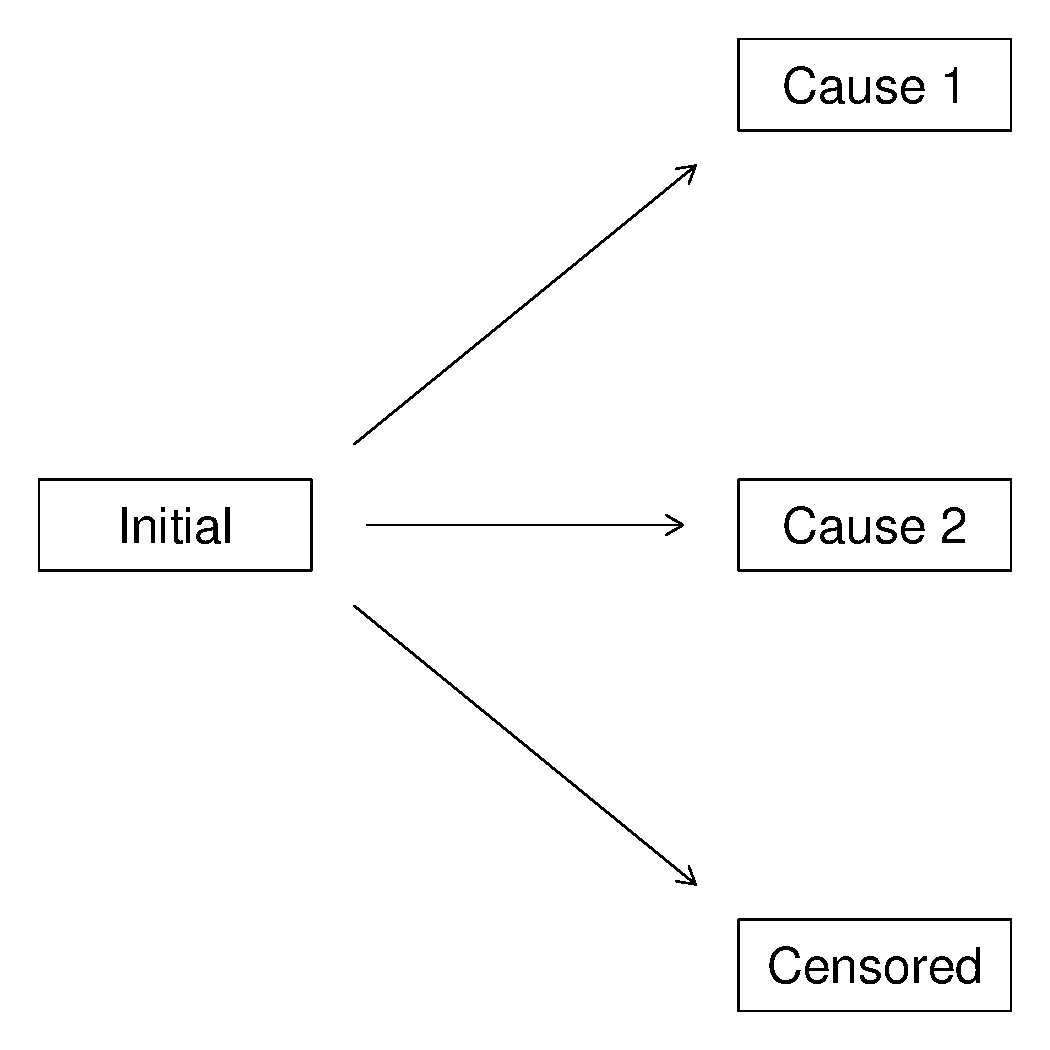
\includegraphics[width=.5\textwidth]{./figure-multi-state-process.pdf}
  \caption{Illustration of the multi-state process \(\eta\) used by
    the state learner. Note that `censored' is a state, hence the
    process is always observed at any time.}
  \label{fig:multi-state-process}
\end{figure}
The conditional distribution of \( \eta(t) \) given \( X=x \) is determined by
the \fxnote*{reconsider letting censoring state be \( -1 \)?}{function}
\begin{equation}
  \label{eq:F-def}
  F(t, k, x) = P(\eta(t) = k \mid X=x),
  \quad \text{for all} \quad
  t \in [0,\tau],
  k \in \{0,1,2,3\},
  x \in \mathcal{X}.
\end{equation}
The function \( F \) describes the conditional state occupation
probabilities corresponding to the observed multi-state process
\(\eta\).

We propose to construct a super learner for \( F \), i.e., the target of this
super learner is $\Psi(P) = F$ where the parameter is identified through
equation~(\ref{eq:F-def}). Because each quadruple
$(\Lambda_{1}, \Lambda_{2}, \Gamma, H)$ characterizes a \(P\in\mathcal P\) which
in turn determines \( (F, H) \), a learner for \( F \) can be constructed from
learners of \( \Lambda_1 \), \( \Lambda_2 \), and $\Gamma$ as follows:
\begin{equation}\label{eq:transition}
  \begin{split}
  F(t, 1, x)
  & = P(\tilde{T} \leq t, \Delta=1 \mid X=x)
    = \int_0^t e^{\{-\Lambda_{1}(s \mid x)-\Lambda_{2}(s \mid x) - \Gamma(s \mid x)\} }  \Lambda_{1}(\diff s \mid x),
  \\
  F(t, 2, x)
  & = P(\tilde{T} \leq t, \Delta=2 \mid X=x)
    = \int_0^t e^{\{-\Lambda_{1}(s \mid x)-\Lambda_{2}(s \mid x) - \Gamma(s \mid x)\} }  \Lambda_{2}(\diff s \mid x),
  \\
  F(t, 3, x)
  & =
    P(\tilde{T} \leq t, \Delta=0 \mid X=x)
    = \int_0^t e^{\{-\Lambda_{1}(s \mid x)-\Lambda_{2}(s \mid x) - \Gamma(s \mid x)\} }  \Gamma(\diff s \mid x),
  \\
  F(t, 0, x)
  &
    = P(\tilde{T} > t \mid X= x)
    = 1- F(t, 1, x) - F(t, 2, x)- F(t, 3, x).
  \end{split}
\end{equation}
The state learner requires three libraries of learners, \(\mathcal{A}_1\),
\( \mathcal{A}_2 \), and \( \mathcal{B} \), where \(\mathcal{A}_1\) and
\( \mathcal{A}_2\) contain learners of the conditional cause-specific cumulative
hazard functions of the event time distribution \(\Lambda_1\) and
\( \Lambda_2\), respectively, and \(\mathcal{B}\) contains learners of the
conditional cumulative hazard function of the censoring
distribution. % We further
% define \(\mathcal{H}\) as the set of all probability distributions on
% \( \mathcal{X} \) and
% \begin{equation*}
%   \mathcal{H}_n=\left\{h\colon\mathcal{O}^n\longrightarrow\mathcal{H} \midd
%     h(\data_n)=H_n = \frac 1 n \sum_{i=1}^n \delta_{X_i} \right\}
% \end{equation*}
% as the library of learners which consists of a single learner, the empirical
% distribution function.
Based on the Cartesian product of
libraries of learners for \((\Lambda_1,\Lambda_2,\Gamma)\) we construct a library
$\mathcal{F}(\mathcal{A}_1, \mathcal{A}_2, \mathcal{B})$ of learners
for \( F \):
\begin{align*}
  \mathcal{F}(\mathcal{A}_1, \mathcal{A}_2, \mathcal{B})
  &= \{ \phi_{a_1,a_2, b} : a_1 \in \mathcal{A}_1, a_2 \in \mathcal{A}_2, b \in \mathcal{B}\},
    \intertext{where in correspondance with  the relations in equation \eqref{eq:transition},} 
    \phi_{a_1,a_2, b}(\data_n)(t,1,x) &= \int_0^t e^{\{-a_1(\data_n)(s \mid x)-a_2(\data_n)(s \mid x) - b(\data_n)(s \mid x)\} }  a_1(\data_n)(\diff s \mid x),\\
  \phi_{a_1,a_2, b}(\data_n)(t,2,x) &= \int_0^t e^{\{-a_1(\data_n)(s \mid x)-a_2(\data_n)(s \mid x) - b(\data_n)(s \mid x)\} }  a_2(\data_n)(\diff s \mid x),\\
  \phi_{a_1,a_2, b}(\data_n)(t,3,x) &= \int_0^t e^{\{-a_1(\data_n)(s \mid x)-a_2(\data_n)(s \mid x) - b(\data_n)(s \mid x)\} }  b(\data_n)(\diff s \mid x),\\
  \phi_{a_1,a_2, b}(\data_n)(t,0,x) &= 1-  \sum_{j=1}^3\phi_{a_1,a_2, b}(\data_n)(t,j,x).
\end{align*}
To evaluate how well a function \( F \) predicts the observed
multi-state process we use the integrated Brier score
\( \bar B_\tau( F,O) = \int_0^{\tau} B_t(F,O) \diff t \), where \( B_t \) is the
Brier score \citep{brier1950verification} at time \( t \in [0, \tau] \),
\begin{equation*}
  B_t(F,O) = \sum_{j=0}^{3}
  \left(
      F(t,j,X) - \1{\{\eta(t)=j\}}
  \right)^2.
\end{equation*}
As described in Section~\ref{sec:super-learning}, each learner
\( \phi_{a_1, a_2, b} \) in the library
\( \mathcal{F}(\mathcal{A}_1, \mathcal{A}_2, \mathcal{B}) \) is evaluated using
the cross-validated loss,
\begin{equation*}
  \hat{R}_{n}(\phi_{a_1,a_2,b} ; \bar{B}_{\tau}) =
  \frac{1}{K}\sum_{k=1}^{K}
  \frac{1}{| \data_n^{k} |}\sum_{O_i \in \data_n^{k}}
  \bar B_\tau
  {
    \left(
      \phi_{a_1,a_2,b}{ (\data_n^{-k})}
      , O_i
    \right)
  },
\end{equation*}
and the discrete state learner is
\begin{align*}\label{eq:discrete-state-learner}
  \hat{\phi}_n
  &=  \argmin_{(a_1,a_2,b)\in \mathcal{A}_1\times\mathcal{A}_2\times\mathcal{B}}
    \hat{R}_{n}(\phi_{a_1,a_2,b} ; \bar{B}_{\tau}).
\end{align*}


\section{Theoretical results for the state learner}
\label{sec:theor-results-prop}

In this section we establish theoretical guarantees for the state learner.
% We let \( \E_P \) denote
% expectation under \( P \) and use \( \Theta \) to denote the
% collection of all conditional state-occupation probability functions.
Proposition~\ref{prop:stric-prop} can be derived from the fact that the
integrated Brier score (also called the continuous ranked probability score) is
a strictly proper scoring rule \citep{gneiting2007strictly}. This implies that
if we minimize the average loss of the integrated Brier score, we recover the
parameters of the data-generating distribution. In particular, the oracle of a
state learner will be consistent if the library of learners contains at least
one learner that is consistent for estimation of \( F \). Recall that the
function \(F\) implicitly depends on the data generating probability measure
\(P\in\mathcal P\) but that this was suppressed in the notation. We now make
this dependence explicit by writing \(F_0\) for the function which is obtained
by substituting a specific \(P_0\in\mathcal{P}\) for \(P\) in equation
\eqref{eq:transition}.

\begin{proposition}
  \label{prop:stric-prop}
  For \(P_0\in\mathcal{P}\) define
  \begin{equation*}
    F^* = \argmin_{F} P_0{[\bar{B}_\tau(F, \blank)]},
  % F^* = \argmin_{(\Lambda_1,\Lambda_2,\Gamma) \in \mathcal{M}\otimes\mathcal{M}\otimes\mathcal{M}} P_0{[\bar B_\tau(\phi_{(\Lambda_1,\Lambda_2,\Gamma)}, \blank)]},
\end{equation*}
where the minimum is taken over all \( F \), such that \( F \) is a conditional
state occupation probability function for some measure \( P \) as defined in equation~(\ref{eq:F-def}).
Then \( F^*(t,j,\blank) = F_0(t,j,\blank) \) \( H \)-almost surely for
any \( j\in \{0,1,2,3\} \) and almost any \( t \in [0, \tau]\).
\end{proposition}
\begin{proof}
  See Appendix~\ref{sec:proof-proposition}.
\end{proof}


We establish a finite sample oracle result for the state learner.
Our Corollary~\ref{cor:oracle-prop} is in essence a special case of a
general cross-validation result by \cite{vaart2006oracle}. We assume
that we split the data into equally sized folds, and for simplicity of
presentation we take \( n \) to be such that
\( |\data_n^{-k}| = n/K \) with \( K \) fixed. We will allow the
number of learners to grow with \( n \) and write
\( \mathcal{F}_n=\mathcal{F}(\mathcal{A}_{1,n}, \mathcal{A}_{2,n},
\mathcal{B}_n)\) as short-hand notation and to emphasize the
dependence on \( n \).
% The discrete super $\hat{\phi}_n$ and the
% oracle $\tilde{\phi}_n$ are defined as in Section~\ref{sec:framework}
% but now with respect to the library \( \mathcal{F}_n \) and the loss
% \( B \).
In the following we let \( \| \blank \|_{P_0} \) denote the norm
\begin{equation}
  \label{eq:norm}
  \| F \|_{P_0} = 
  \left\{
    \sum_{j=0}^{3}\int_{\mathcal{X}} \int_0^{\tau} F(t, j, x)^2 \diff t H_0( \diff x)
  \right\}^{1/2}.
\end{equation}
\begin{corollary}
  \label{cor:oracle-prop}
  For all \(P_0\in\mathcal{P}\), \( n \in \N \), \( k \in \{1, \dots, K\} \),
  and $\delta>0$,
  \begin{align*}
    \E_{P_0}{\left[ \Vert \hat{\phi}_n(\data_n^{-k}) - F_0 \Vert_{P_0}^2 \right]}
    & \leq (1 + 2\delta)
      \E_{P_0}{\left[ \Vert \tilde{\phi}_n(\data_n^{-k}) - F_0 \Vert_{P_0}^2 \right]}
    \\
    & \quad
      + (1+ \delta) 16   K \tau
      \left(
      13 + \frac{12}{\delta}
      \right)
      \frac{\log(1 + |\mathcal{F}_n|)}{n}.
  \end{align*}
\end{corollary}
\begin{proof}
  See Appendix~\ref{sec:proof-proposition}.
\end{proof}

Corollary~\ref{cor:oracle-prop} has the following asymptotic consequences.

\begin{corollary}
  \label{cor:asymp-cons}
  Assume that \( |\mathcal{F}_n| = \bigO(n^q)\), for some \( q \in \N \)
  and that there exists a sequence \( \phi_n \in \mathcal{F}_n \),
  \( n \in \N \), such that
  \( \E_{P_0}{\left[ \Vert \phi_n(\data_n^{-k}) - F_{0} \Vert_{P_0}^2 \right]} =
  \bigO(n^{-\alpha}) \), for some \( \alpha\leq 1 \).
  \begin{enumerate}[label=(\roman*), topsep=0pt]
  \item If $\alpha=1$ then
    \( \E_{P_0}{\left[ \Vert \hat{\phi}_n(\data_n^{-k}) - F_0 \Vert_{P_0}^2
      \right]} = \bigO(\log(n)n^{-1}) \).
  \item If $\alpha<1$ then
    \( \E_{P_0}{\left[ \Vert \hat{\phi}_n(\data_n^{-k}) - F_0 \Vert_{P_0}^2 \right]} =
    \bigO(n^{-\alpha}) \).
  \end{enumerate}
\end{corollary}
\begin{proof}
  See Appendix~\ref{sec:proof-proposition}.
\end{proof}

In Section~\ref{sec:targeted-learning} we demonstrate how the state learner can
be used for targeted learning. A targeted estimator is typically obtained from
estimators of the nuisance parameters $\Lambda_1$, $\Lambda_2$, and $\Gamma$. By
equations~(\ref{eq:lambdaj}) and~(\ref{eq:gamma}) and the definition of \( F \),
we have
\begin{equation}
  \label{eq:7}
  \Gamma(t , x) 
  = \int_0^t  \frac{F(\diff s, 3, x )}{F(s-, 0, x )},
  \quad \text{and} \quad
  \Lambda_j(t , x) 
  = \int_0^t  \frac{F(\diff s, j, x )}{F(s-, 0, x )},
  \quad j \in \{1,2\},
\end{equation}
and thus a targeted estimator can also be obtained from an estimator of $F$
using equation~(\ref{eq:7}). The key feature of a targeted estimator is that it
is asymptotically equivalent to a sum of i.i.d.\ random variables plus a second
order remainder term \citep{bickel1993efficient,fisher2021visually}. For our
setting of competing risks, the remainder term is typically dominated by terms
of the form
\begin{equation}
  \label{eq:dr-term}
  P{\left[
      \int_0^{\tau} w_n(s, \blank)
      \hat{M}_{1,n}(s \mid  \blank)
      \hat{M}_{2,n}(\diff s \mid  \blank)
    \right]},
\end{equation}
where \( (\hat{M}_{1,n}, \hat{M}_{2,n}) \) is any of the nine combinations of
\( \hat{M}_{1,n} \in \{[\Gamma -\hat{\Gamma}_n], [\Lambda_1
-\hat{\Lambda}_{1,n}], [\Lambda_2 -\hat{\Lambda}_{2,n}]\} \) and
\( \hat{M}_{2,n} \in \{[\Gamma -\hat{\Gamma}_n], [\Lambda_1
-\hat{\Lambda}_{1,n}], [\Lambda_2 -\hat{\Lambda}_{2,n}]\} \), and \( w_n \) is
some data-dependent function with domain \([0,\tau]\times\mathcal X \)
\citep{van2003unified}. In particular, a targeted estimator will be
asymptotically linear if the `products' of the estimation errors
\( \hat{M}_{1,n} \) and \( \hat{M}_{2,n} \) in equation~(\ref{eq:dr-term}) are
\( \smallO_P{(n^{-1/2})}\). Proposition~\ref{prop:dr-structure} states that if
equation~(\ref{eq:dr-term}) holds for the a targeted estimator based on
estimators $\hat{\Lambda}_{1,n}$, $\hat{\Lambda}_{2,n}$, and $\hat{\Gamma}_{n}$,
then a similar product structure holds for a targeted estimator based on
\( \hat{F}_n \). We state the result for the special case that
\(\hat{M}_{1,n}= \Gamma-\hat{\Gamma}_n \) and
\(\hat{M}_{2,n} =\Lambda_1-\hat{\Lambda}_{1,n} \), but similar results holds for
any combinations of \( \Gamma-\hat{\Gamma}_n\),
\( \Lambda_1-\hat{\Lambda}_{1,n} \), and \( \Lambda_2-\hat{\Lambda}_{2,n} \).
\begin{proposition}
  \label{prop:dr-structure}
  Assume that \( w(s,x)\leq c \), \( F(s, 0, x) \geq 1/c \) and
  \( \hat{F}_n(s, 0, x) \geq 1/c \) for some \( c>0 \) for all
  \( s \in [0, \tau] \) and \( x \in \mathcal{X} \). Then there are real-valued
  uniformly bounded functions \( w^a_n \), \( w^b_n \), \( w^c_n \), and
  \( w^d_n \) with domain \( [0,\tau]^2 \times \mathcal{X} \) such that
  \begin{align*}
    & P_0{\left[
      \int_0^{\tau} w(s, \blank)
      \left\{
      \Gamma_0(s,\blank) -\hat{\Gamma}_n(s,\blank)
      \right\}
      [\Lambda_0-\hat{\Lambda}_n]
      (\diff s, \blank)
      \right]}
    \\
    & =
      P_0{\left[
      \int_0^{\tau} \int_0^{s} w^a_n(s,u,\blank) [F_0 - \hat{F}_n](u-, 0, \blank)[F_0 - \hat{F}_n](s-, 0, \blank) F_0(\diff u, 2, \blank ) F_0 ( \diff s, 1, \blank)
      \right]}
    \\
    & \quad +
      P_0{\left[
      \int_0^{\tau} \int_0^{s} w^b_n(s,u,\blank) [F_0 - \hat{F}_n](u-, 0, \blank)
      F_0(\diff u, 2, \blank ) [F_0 - \hat{F}_n](\diff s, 1, \blank)
      \right]}
    \\
    & \quad +
      P_0{\left[
      \int_0^{\tau} \int_0^{s} w^c_n(s,u,\blank) [F_0 - \hat{F}_n](\diff u, 2, \blank)
      [F_0 - \hat{F}_n](s-, 0, \blank)
      F_0(\diff s, 1, \blank ) 
      \right]}
    \\
    & \quad +
      P_0{\left[
      \int_0^{\tau} \int_0^{s} w^d_n(s,u,\blank) [F_0 - \hat{F}_n](\diff u, 2, \blank)
      [F_0 - \hat{F}_n](\diff s, 1, \blank)
      \right]}.
  \end{align*}
\end{proposition}
\begin{proof}
  See Appendix~\ref{sec:state-learner-with}.
\end{proof}

\section{Targeted learning}
\label{sec:targeted-learning}

Features of the observed data distribution \( P \in \mathcal{P} \) are rarely of
interest. We are instead interested in a parameter
\( \theta \colon \mathcal{Q} \rightarrow \Theta \) that expresses a property of
the uncensored population governed by the measure \( Q \in \mathcal{Q} \). The
parameter space $\Theta$ can be a subset of \(\R^d\) or a subset of a function
space, such as \(\mathcal{M}\). In subsection~\ref{sec:cause-spec-aver} we give
a concrete example from causal inference where $\theta$ is the average treatment
effect and \( \Theta = [-1,1] \). Under the assumption of conditional
independent censoring and positivity, $\theta$ is identifiable from
\( \mathcal{P} \) which means that there exists an operator
\( \Psi \colon \mathcal{P} \rightarrow \Theta \) such that
\( \theta(Q) = \Psi(P_{Q, \Gamma}) \) for all $\Gamma \in \mathcal{M}$. By
equation~(\ref{eq:parametrizeP}) this imply that we may write
\begin{equation*}
  \theta(Q) = \Psi(P) = \tilde{\Psi}^0(\Lambda_1, \Lambda_2, H),
\end{equation*}
for some operator \( \tilde{\Psi}^0 \). The state learner provides a ranking of
tuples
\( (a_1, a_2, b) \in \mathcal{A}_1 \times \mathcal{A}_2 \times \mathcal{B} \),
and we use \( \hat{a}_{1,n} \), \( \hat{a}_{2,n} \), and \( \hat{b}_n \) to
denote the learners corresponding to the discrete state learner
\( \hat{\phi}_n \). Letting \( H(\data_n) \) denote the empirical measure of
\( \{X_1, \dots, X_n\} \), we can obtain a simple plug-in an estimator of
$\theta$ as
\begin{equation}
  \label{eq:2}
  \hat{\Psi}^0(\data_n) =
  \tilde{\Psi}^0(\hat{a}_{1,n}(\data_n), \hat{a}_{2,n}(\data_n), H(\data_n)). 
\end{equation}

The asymptotic distribution of \( \hat{\Psi}_{\tau, j}^0 \) is difficult to
analyze due to the model selection step involved when estimating the nuisance
parameters $\Lambda_1$ and $\Lambda_2$. In addition, the estimator will
typically have an asymptotic bias that vanishes at a sub-optimal rate. Using
tools from semi-parametric efficiency theory, it is possible to construct a
so-called targeted or debiased estimator with smaller asymptotic bias and an
asymptotic distribution which we know how to estimate
\citep{bickel1993efficient,van2011targeted,chernozhukov2018double}. A targeted
estimator is based on the efficient influence function for the parameter
$\tilde{\Psi}^0$ and relies on an estimator of $\Gamma$ in addition to
estimators of \( \Lambda_1 \) and $\Lambda_2$. The efficient influence function
is a \( P \)-zero mean and square integrable function indexed by the nuisance
parameters \( (\Lambda_1, \Lambda_2, \Gamma) \), which we denote by
\( \psi(\blank ; \Lambda_1, \Lambda_2, \Gamma) \). The name is justified because
any regular asymptotically linear estimator that has \( \psi \) as its influence
function is efficient, meaning that it has smallest asymptotic variance among
all regular asymptotically linear estimators.

An example of a targeted estimator is the one-step estimator, defined as
\begin{equation}
    \label{eq:one-step-def}
    \hat{\Psi}_{\text{OS}}(\data_n)
    =
    \tilde{\Psi}^0(\hat{a}_{1,n}(\data_n), \hat{a}_{2,n}(\data_n),
    H(\data_n))
    + \empmeas{[\psi(\blank; \hat{a}_{1,n}(\data_n), \hat{a}_{2,n}(\data_n),
      \hat{b}_n(\data_n) )]},
\end{equation}
where \( \empmeas \) is the empirical measure of a sample \(\{O_i\}_{i=1}^n\).
We can make the following asymptotic expansion of the one-step estimator
\citep{pfanzagl1985contributions,van2003unified,fisher2021visually,kennedy2022semiparametric,rytgaard2022continuous},
\begin{equation*}
  \hat{\Psi}_{\text{OS}}(\data_n)- \Psi(P)
  =  \empmeas{[\psi(\blank ; \Lambda_1, \Lambda_2, \Gamma)]}
  +\mathrm{Rem}{(\hat{\Lambda}_{1,n},\hat{\Lambda}_{2,n},  \hat{\Gamma}_n, P)} + \smallO_{P}(n^{-1/2}),
\end{equation*}
where the remainder term is typically such that
\begin{equation}
  \label{eq:4}
  \mathrm{Rem}{(\hat{\Lambda}_{1,n},\hat{\Lambda}_{2,n},  \hat{\Gamma}_n, P)}
  = \mathcal{O}_P{
    \left\{
      \|\Lambda_1-\hat{\Lambda}_{1,n}\|^2
      +
      \|\Lambda_2-\hat{\Lambda}_{2,n}\|^2
      +
      \|\Gamma-\hat{\Gamma}_{n}\|^2
    \right\}
  },
\end{equation}
for some suitable norm \( \|\blank \| \), for instance the
\( \mathcal{L}_{P}^2 \)-norm. Hence, under a suitable Donsker class regularity
condition \citep{bickel1993efficient,kennedy2016semiparametric}, when
equation~(\ref{eq:4}) holds and the nuisance parameters $\Lambda_1$,
$\Lambda_2$, and $\Gamma$ are consistently estimated at rate
\( \smallO_P{(n^{-1/4})} \), then
\begin{equation}
  \label{eq:3}
  \sqrt{n}(\hat{\Psi}_{\text{OS}}(\data_n)- \Psi(P)) \weakly \mathcal{N}(0,
  P{[\psi(\blank; \Lambda_1, \Lambda_2, \Gamma)^2]}),
\end{equation}
where we use \( \weakly \) to denote weak convergence \citep{van2000asymptotic}.
In particular, equation~(\ref{eq:3}) and Slutsky's lemma imply that we can
obtain asymptotically valid \((1-\alpha)\cdot100\%\) confidence intervals by
calculating
\begin{equation*}
  \left[
    \hat{\Psi}_{\text{OS}}(\data_n) - q_{\alpha/2} \hat{\sigma}(\data_n) ,
    \;
    \hat{\Psi}_{\text{OS}}(\data_n) + q_{\alpha/2} \hat{\sigma}(\data_n)
  \right],
\end{equation*}
where \( q_{\alpha} \) is the \( (1-\alpha) \)-quantile or the standard normal
distribution, and
\begin{equation*}
  \hat{\sigma}(\data_n) = 
  \left(
    \empmeas{
      \left[
        \psi(\blank; \hat{a}_{1,n}(\data_n), \hat{a}_{2,n}(\data_n),
        \hat{b}_n(\data_n))^2
      \right]}
  \right)^{1/2}.
\end{equation*}


\subsection{Average treatment effect on the cumulative incidence}
\label{sec:cause-spec-aver}

In the following we demonstrate how the state learner and the general estimation
strategy outlined above can be used to construct an estimator of the
cause-specific average treatment effect. We assume that the covariate vector
\( X \in \R^p \) can be separated into a binary treatment indicator \( A \) and
a vector of potential confounders, \( W \in \mathcal{W}\subset \R^{p-1} \). We
abuse notation slightly by writing
\( \Lambda_j(t \mid x) = \Lambda_j(t \mid a, w) \) and
\( S(t \mid x) = S(t \mid a, w) \) when \( x=(a, w) \). We use $\mu$ to denote
the marginal distribution of \( W \) and $\pi$ to denote the conditional
probability of treatment,
\begin{equation*}
  \pi(w) = P(A=1 \mid W=w).
\end{equation*}
We assume throughout that $\pi$ is uniformly bounded away from \( 0 \) and
\( 1 \) on \( \mathcal{W} \). As both \( A \) and \( W \) are fully observed for
all individuals we can use an existing super learner to estimate $\pi$
\citep{Polley_Ledell_Kennedy_Laan_2023_Superlearn}, and we denote this estimator
by $\hat{\pi}_n$. We use the empirical measure of \( \{W_1, \dots, W_n\} \) to
estimate $\mu$, and denote this estimator by the $\hat{\mu}_n$. As parameter of
interest we consider the standardized difference in the cumulative incidence due
to cause 1 at time $\tau$, which can be expressed as
\begin{equation*}
  \theta_{{\tau}}(Q) = \int_{\mathcal{W}} 
  \left\{
    \int_0^{\tau}
    S(s- \mid w, 1)  \Lambda_1(\diff s \mid w, 1)
    -
    \int_0^{\tau}
    S(s- \mid w, 0)  \Lambda_1(\diff s \mid w, 0)
  \right\}
  \mu(\diff w).
\end{equation*}
Under a set of
additional assumptions, \( \theta_{{\tau}} \) can be given the causal
interpretation
\begin{equation*}
  \theta_{{\tau}}(Q) =
  P{(T^{A=1} \leq \tau, D^{A=1}=1)}-
  P{(T^{A=0} \leq \tau, D^{A=0}=1)},
\end{equation*}
where \( (T^A, D^A) \) denotes potential outcomes \citep{hernanRobinsWhatIf}. In
this case, the interpretation of $\theta_{\tau}$ is the difference in the
average risk of cause \( 1 \) occurring before time \( \tau \) in the population
if everyone had been given treatment (\( A=1 \)) compared to if no one had been
given treatment.

Using equation~(\ref{eq:surv-def}), we may write
\( \theta_{{\tau}}(Q) = \tilde{\Psi}_{t}^0(\Lambda_1, \Lambda_2, \mu) \),
where
\begin{equation}
  \label{eq:1}    
  \begin{split}
  \tilde{\Psi}_{t}^0(\Lambda_1, \Lambda_2, \mu) & =
  \int_{\mathcal{W}} 
  \int_0^{\tau}
  e^{-\Lambda_1(s- \mid w, 1)-\Lambda_2(s- \mid w, 1)}  \Lambda_1(\diff s \mid
  w, 1)
  \mu(\diff w)
  \\
  &  \quad
  -\int_{\mathcal{W}} 
  \int_0^{\tau}
  e^{-\Lambda_1(s- \mid w, 0)-\Lambda_2(s- \mid w, 0)}  \Lambda_1(\diff s \mid w, 0)
  \mu(\diff w).
  \end{split}
\end{equation}
The efficient influence function for the parameter $\tilde{\Psi}_{\tau}$ depends
on the set \( (\Lambda_1, \Lambda_2, \Gamma, \pi) \) of nuisance parameters.
Define the quantities
\begin{align*}
  \omega_a(A,W; \pi)
  &=  \frac{% (-1)^{a+1}
    \1{\{A=a\}}}{\pi(W)^{a}(1-\pi(W))^{1-a}},
  \\
  g(t, A, W; \Lambda_1, \Lambda_2)
  & = \int_0^{t}
    e^{-\Lambda_1(s- \mid W, A)-\Lambda_2(s- \mid W, A)}  \Lambda_1(\diff s \mid
    W, A),
  \\  
  M_j(\diff t \mid A, W;  \Lambda_j  )
  & = N_j(\diff t) -
    \1{\{\tilde{T} \geq t\}} \Lambda_j(\diff t \mid W, A),
    \quad j \in \{1,2\},
  \intertext{and}
  M(\diff t \mid A, W;  \Lambda_1, \Lambda_2  )
  & = M_1(\diff t \mid A, W;  \Lambda_1  ) +
    M_2(\diff t \mid A, W;  \Lambda_2  ).
\end{align*}
The efficient influence function can then be written as
\citep{van2003unified,jewell2007non,rytgaard2022targeted},
\begin{equation*}
  \psi_{\tau}(O; \Lambda_1, \Lambda_2, \Gamma, \pi)
  = \psi_{\tau}^1(O; \Lambda_1, \Lambda_2, \Gamma, \pi)
  - \psi_{\tau}^0(O; \Lambda_1, \Lambda_2, \Gamma, \pi)
  -\tilde{\Psi}_{t}^0(\Lambda_1, \Lambda_2, \mu),
\end{equation*}
where
\begin{equation}
  \label{eq:5}
  \begin{split}
    & \psi_{\tau}^a(O; \Lambda_1, \Lambda_2, \Gamma, \pi)
    \\
    & =
      \omega_a(A,W; \pi)
      \int_0^{\tau} e^{\Gamma(t- \mid A, W)}   
      M_1(\diff t \mid A, W; \Lambda_1)
    \\
    & \quad
      -
      \omega_a(A,W; \pi)
      g(\tau, A, W; \Lambda_1, \Lambda_2)
      \int_0^{\tau}
      e^{[\Gamma+\Lambda_1 + \Lambda_2](t- \mid A, W)}
      M(\diff t \mid A, W; \Lambda_1, \Lambda_2)
    \\
    & \quad
      +
      \omega_a(A,W; \pi)      
      \int_0^{\tau}
      g(t, A, W; \Lambda_1, \Lambda_2)
      e^{[\Gamma+\Lambda_1 + \Lambda_2](t- \mid A, W)}
      M(\diff t \mid A, W; \Lambda_1, \Lambda_2)
    \\
    & \quad + g(\tau, a, W; \Lambda_1, \Lambda_2).
  \end{split}
\end{equation}

Equations~(\ref{eq:1}) and~(\ref{eq:5}) allow us to construct a one-step
estimator by using the definition given in equation~(\ref{eq:one-step-def}),
which gives the estimator
\begin{equation}
  \label{eq:one-step-comp-ate}
  \begin{split}
    \hat{\Psi}_{t,\text{OS}}(\data_n)
    = &
        \tilde{\Psi}_{t}^0(\hat{a}_1(\data_n), \hat{a}_2(\data_n),
        \hat{\mu}_n(\data_n))
    \\
      &
        +
        \empmeas{[\psi_{\tau}(\blank; \hat{a}_{1,n}(\data_n), \hat{a}_{2,n}(\data_n),
        \hat{b}_n(\data_n), \hat{\pi}_n(\data_n))]}
    \\
    = &
        \empmeas{[\psi_{\tau}^1(\blank; \hat{a}_{1,n}(\data_n), \hat{a}_{2,n}(\data_n),
        \hat{b}_n(\data_n), \hat{\pi}_n(\data_n))]}
    \\
      &
        - \empmeas{[\psi_{\tau}^0(\blank; \hat{a}_{1,n}(\data_n), \hat{a}_{2,n}(\data_n),
        \hat{b}_n(\data_n), \hat{\pi}_n(\data_n))]}.
  \end{split}
\end{equation}


\section{Numerical experiments}
\label{sec:numer-exper}

As a proof of concept we conduct two small simulation studies in a setting
without competing risks. We generate data according to a distribution motivated
from a real dataset in which censoring depends on the baseline covariates. We
simulate data based on a prostate cancer study described in
\citep{kattan2000pretreatment}. The outcome of interest was the time to tumor
recurrence, and five baseline covariates were used to predict outcome:
prostate-specific antigen (PSA, ng/mL), Gleason score sum (GSS, values between 6
and 10), radiation dose (RD), hormone therapy (HT, yes/no) and clinical stage
(CS, six values). The study was designed such that a patient's radiation dose
depended on when the patient entered the study \citep{gerds2013estimating}. This
in turn implied that the time of censoring depended on the radiation dose. The
data were re-analyzed in \citep{gerds2013estimating} where a sensitivity
analysis was conducted based on simulated data. We use the same simulation
setup, where event and censoring times are generated according to parametric
Cox-Weibull models estimated from the original data, and the covariates are
generated according to either marginal Gaussian normal or binomial distributions
estimated from the original data
\citep[c.f.,][Section~4.6]{gerds2013estimating}. We refer to this simulation
setting as ``dependent censoring''. We also considered a simulation setting
where data were generated in the same way, except that censoring was generated
completely independently. We refer to this simulation setting as ``independent
censoring''.

For all super learners we use a library consisting of three learners: The
Kaplan-Meier estimator \citep{kaplan1958nonparametric,Gerds_2019prodlim}, a Cox
model with main effects \citep{cox1972regression, survival-package}, and a
random survival forest \citep{ishwaran2008random,rfsrc-paclage}. We use the same
library to learn the outcome and the censoring mechanism. To be precise, note
that given a learner for the cumulative hazard function of the outcome event, we
can typically use the same method to construct a learner of the cumulative
hazard function of the censoring distribution. This would typically work by
training the learner on the data set \( \data_n^c \), where
\( \data_n^c = \{O_i^c\}_{i=1}^n \) with
\( O_i^c = (\tilde{T}_i, 1-\Delta, X_i) \). When we say that we use a learner
for the cumulative hazard function of the outcome to learn the cumulative hazard
function of the censoring time, we mean that the learner is trained on
\( \data_n^c \).

We first compare the state learner to two IPCW based super learners: The first
uses a Cox model with main effects to estimate the censoring probabilities
(IPCW(Cox)), while the second uses the Kaplan-Meier estimator to estimate the
censoring probabilities (IPCW(KM)). The Cox model for the censoring distribution
is correctly specified in both simulation settings while the Kaplan Meier
estimator only estimates the censoring model correctly in the simulation setting
where censoring is independent. Both IPCW super learners are fitted using the
\texttt{R}-package \texttt{riskRegression} \citep{Gerds_Ohlendorff_Ozenne_2023}.
Each super learner provides a learner for the cumulative hazard function for the
outcome of interest, and from this a risk prediction model can be obtained. We
measure performance of each super learner by calculating the index of prediction
accuracy (IPA) \citep{kattan2018index} at a fixed time horizon (36 months) for
the risk prediction model provided by the super learner. The IPA is 1 minus the
ratio between the model's Brier score and the null model's Brier score, where
the null model is the model that does not use any covariate information. The IPA
is approximated using a large (\( n = 20,000 \)) independent data set of
uncensored data. As a benchmark we calculate the performance of the risk
prediction model chosen by the oracle selector. The oracle selector uses the
large data set of uncensored event times to select the learner with the highest
IPA.

The results are shown in Figure~\ref{fig:ipcw-fail}. We see that when censoring
is not independent, using the Kaplan-Meier estimator to estimate the censoring
probabilities provides a risk prediction model with an IPA that is lower than
the risk prediction model provided by the state learner. The performance of the
risk prediction model selected by the state learner is similar to the risk
prediction model selected by the IPCW(Cox) super learner which a priori uses a
correctly specified model for the censoring distribution. Both these risk
prediction models are close to the performance of the oracle, except for small
sample sizes.

\begin{figure}
  \centerline{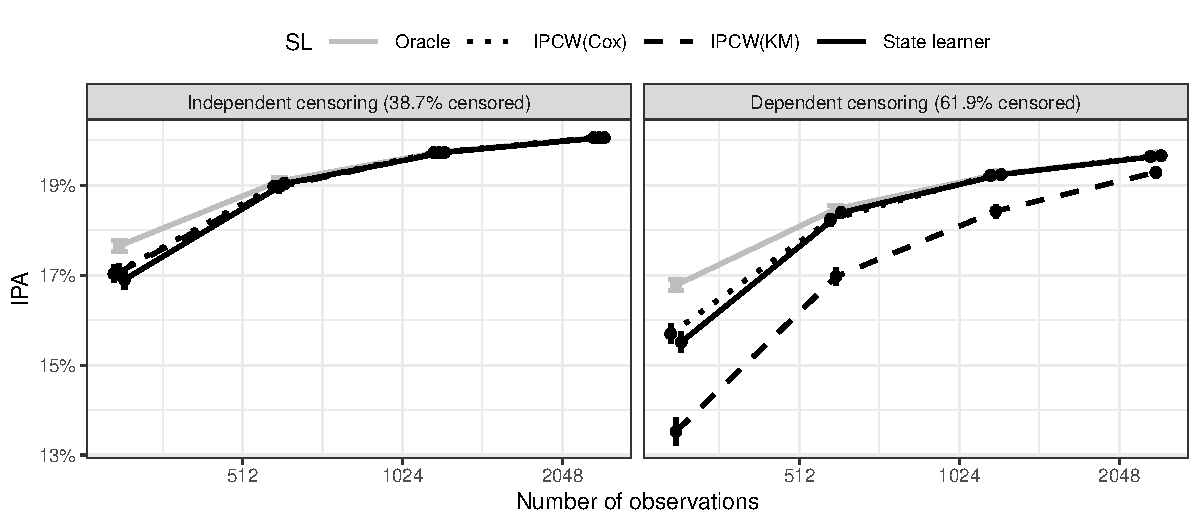
\includegraphics[width=1\linewidth]{./experiment-fig-sl-ipcw.pdf}}
  \caption[]{For the risk prediction models provided by each of the super
    learners, the IPA is plotted against sample size. The results are based on
    1000 repetitions and the error bars are used to quantify the Monte Carlo
    uncertainty.}
  \label{fig:ipcw-fail}
\end{figure}

We next compare the state learner to the super learner \texttt{survSL}
\citep{westling2021inference}, as this is the only existing super learner we
know which works without a pre-specified censoring model. As both the state
learner and \texttt{survSL} also provides a prediction model for the probability
of being censored, we compare the performance of both the outcome and the
censoring modeling using the IPA.

The results are shown in Figure~\ref{fig:zelefski}. We see that the prediction
models selected for both censoring and outcome have similar or higher API
compared to the prediction models selected by \texttt{survSL} for most sample
sizes.

\begin{figure}
  \centerline{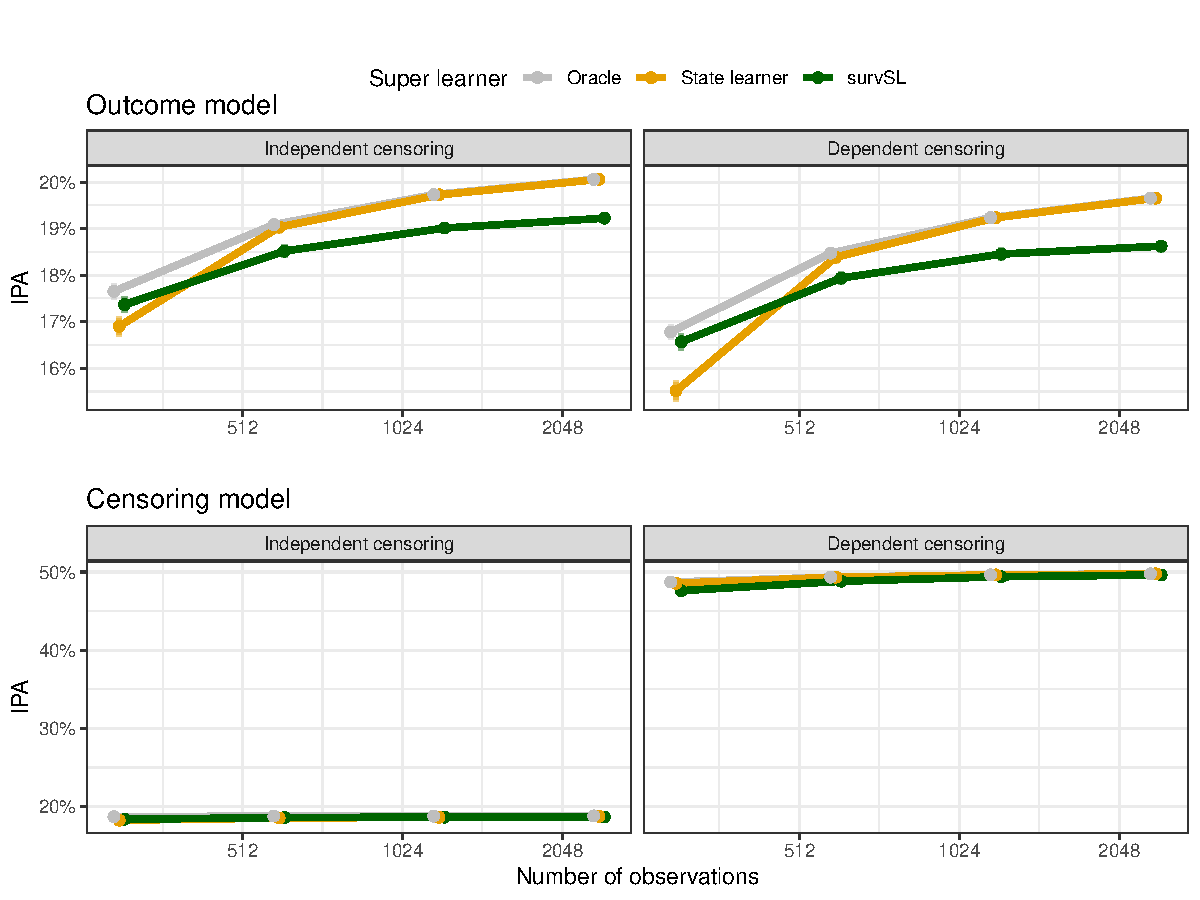
\includegraphics[width=1\linewidth]{./experiment-fig-sl-survSL.pdf}}
  \caption[]{For the risk prediction models of both the outcome and the
    censoring probability provided by each of the super learners, the IPA is
    plotted against sample size. The results are based on 1000 repetitions and
    the error bars are used to quantify the Monte Carlo uncertainty.}
  \label{fig:zelefski}
\end{figure}


\section{Example with prostate cancer study}
\label{sec:real-data-appl}

The prostate cancer data analyzed by \cite{kattan2000pretreatment}, which we
introduced in Section~\ref{sec:numer-exper}, include a competing event in the
form of death without tumor recurrence. For illustration, we fit the state
learner to the original data set consisting of 1,042 patients. We consider death
without tumor recurrence and recurrence of tumor as two competing events of
interest. We include the fives learner \texttt{KM}, \texttt{Cox strata CS},
\texttt{Lasso}, \texttt{Elastic}, and \texttt{RF} which are described in
Table~\ref{tab:zel-library}. We use the same library of learners to learn
\( \Lambda_1 \), \( \Lambda_2 \), and $\Gamma$. In this case, \( \Lambda_1 \)
denotes the cause-specific cumulative hazard function of tumor recurrence, and
\( \Lambda_2 \) denotes the cause-specific cumulative hazard function of death
without tumor recurrence.

\begin{table}
  \caption{\label{tab:zel-library}Overview of the five learners used by the
  state learner when applied to the prostate cancer data set. The Kaplan-Meier
  estimator was fitted using the package \texttt{prodlim}
  \citep{Gerds_2019prodlim}. All Cox models included all five covariates in
  the model and were fitted using the package \texttt{survival}
  \citep{survival-package}. All penalized Cox models included all five
  covariates as linear predictors and were fitted using the package
  \texttt{glmnet} \citep{glmnet-cox,glmnet-glm}. The random forest was fitted
  with the package \texttt{randomForestSRC} \citep{rfsrc-paclage}.}
\centering
  \begin{tabular}{ lll }
    \toprule
    Family & Model & Description \\
    \midrule
    Marginal & \texttt{KM} & The Kaplan-Meier estimator \\ 
    Cox & \texttt{Cox} & All five covariates included with additive effects \\
           & \( \texttt{Cox strata CS} \)  & Cox model stratified on CS  \\
           % & \( \texttt{Cox strata HT} \)  & Cox model stratified on HT \\
           % & \( \texttt{Cox spline} \)  & PSA and RD modeled with splines \\ 
    Penalized Cox & \texttt{Lasso} & Cox model with \( L_1 \)-norm penalty   \\
           % & \texttt{Ridge} & Cox model with \( L_2 \)-norm penalty \\
           & \texttt{Elastic} & Cox model with \( L_1 \)- and \( L_2 \)-norm penalty \\
    Random forest & \texttt{RF} & Random forest with default settings \\
    \bottomrule 
  \end{tabular}
\end{table}


This gives a library consisting of \( 5^3 = 125 \) learners for the conditional
state occupation probability function \( F \) defined in
equation~(\ref{eq:F-def}). We use five folds for training and testing the
models, and we repeat training and evaluation five times with different splits.
The integrated Brier score (defined in Section~\ref{sec:super-learner-simple})
for all learners are shown in Figure~\ref{fig:zelefski-real}, and the top 10
combinations of learners are displayed in Table~\ref{tab:zelefski-real}. We see
that the prediction performance is mostly affected by the choice of learner for
the censoring distribution. Several combinations of learners give similar
performance as measured by the integrated Brier score, as long as a random
forest is used to model the censoring distribution.

\begin{figure}
  \centerline{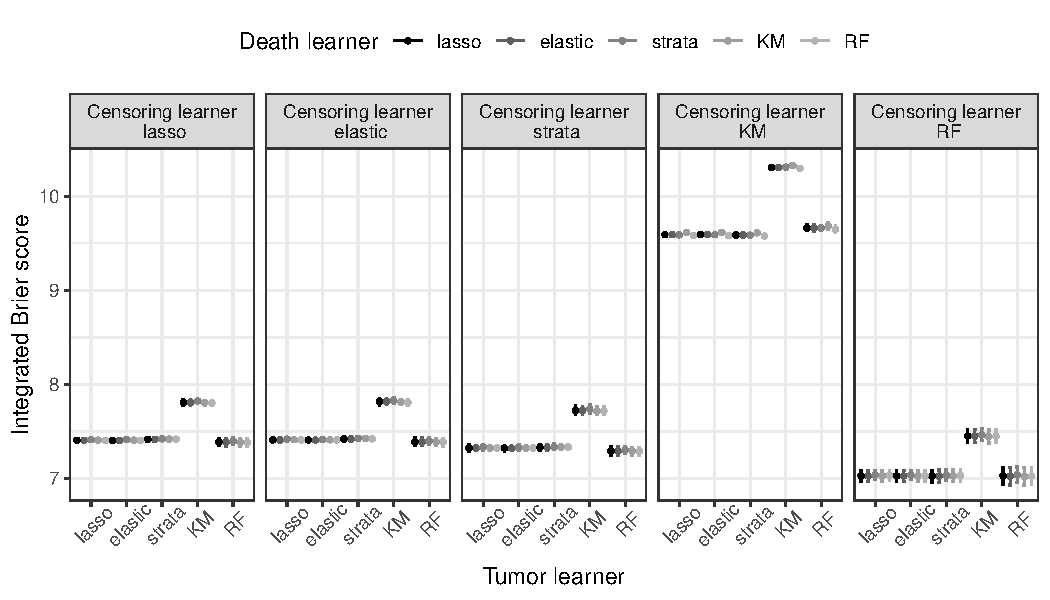
\includegraphics[width=1\linewidth]{./zelefski-real-data.pdf}}
  \caption[]{The results of applying the 125 combinations of learners to the
    prostate cancer data set. The learners are \texttt{KM} (KM), \texttt{Cox
      strata CS} (strata), \texttt{Lasso} (lasso), \texttt{Elastic} (elastic),
    and \texttt{RF} (RF) as described Table~\ref{tab:zel-library}. The error
    bars are based on five repetitions using different splits. We refer to
    learners of \( \Lambda_1 \), \( \Lambda_2 \), and $\Gamma$ as `Tumor
    learner', `Death learner', and `Censoring learner', respectively.}
  \label{fig:zelefski-real}
\end{figure}


\begin{table}
  \caption{\label{tab:zelefski-real}The 10 best performing models in terms of integrated Brier score. The
    reported standard errors are based on five repetitions using different
    splits. The models are described in Table~\ref{tab:zel-library}. We refer to
    learners of \( \Lambda_1 \), \( \Lambda_2 \), and $\Gamma$ as `Tumor
    learner', `Death learner', and `Censoring learner', respectively.}
  \centering
  % latex table generated in R 4.0.3 by xtable 1.8-4 package
% Thu Aug 24 20:38:52 2023
\begin{tabular}{lll|l}
  \toprule
Tumor learner & Death learner & Censoring learner & Integrated Brier score \\ 
  \midrule
\texttt{Elastic} & \texttt{Elastic} & \texttt{RF} & $7.03\pm0.02$ \\ 
  \texttt{Elastic} & \texttt{KM} & \texttt{RF} & $7.03\pm0.02$ \\ 
  \texttt{Lasso} & \texttt{Elastic} & \texttt{RF} & $7.04\pm0.02$ \\ 
  \texttt{Lasso} & \texttt{KM} & \texttt{RF} & $7.04\pm0.02$ \\ 
  \texttt{Elastic} & \texttt{Lasso} & \texttt{RF} & $7.04\pm0.02$ \\ 
  \texttt{Cox strata CT} & \texttt{Elastic} & \texttt{RF} & $7.04\pm0.03$ \\ 
  \texttt{Lasso} & \texttt{Lasso} & \texttt{RF} & $7.04\pm0.02$ \\ 
  \texttt{Cox strata CT} & \texttt{Lasso} & \texttt{RF} & $7.04\pm0.03$ \\ 
  \texttt{Cox strata CT} & \texttt{KM} & \texttt{RF} & $7.04\pm0.03$ \\ 
  \texttt{Elastic} & \texttt{RF} & \texttt{RF} & $7.04\pm0.02$ \\ 
   \bottomrule
\end{tabular}

\end{table}



As an illustration, we use the learners of the three cumulative hazard functions
selected by the state learner and the estimator defined in
Section~\ref{sec:cause-spec-aver}, equation~(\ref{eq:one-step-comp-ate}), to
estimate the average treatment effect of hormone therapy on risk of tumor
recurrence and death. The results are shown in
Figure~\ref{fig:zelefski-real-target} for 6 month intervals after baseline with
point wise 95\% confidence intervals. We see that hormone therapy appears to
decrease the risk of tumor recurrence and increase the risk of death without
tumor recurrence, but that not of the estimated effects are significant.

\begin{figure}
  \centerline{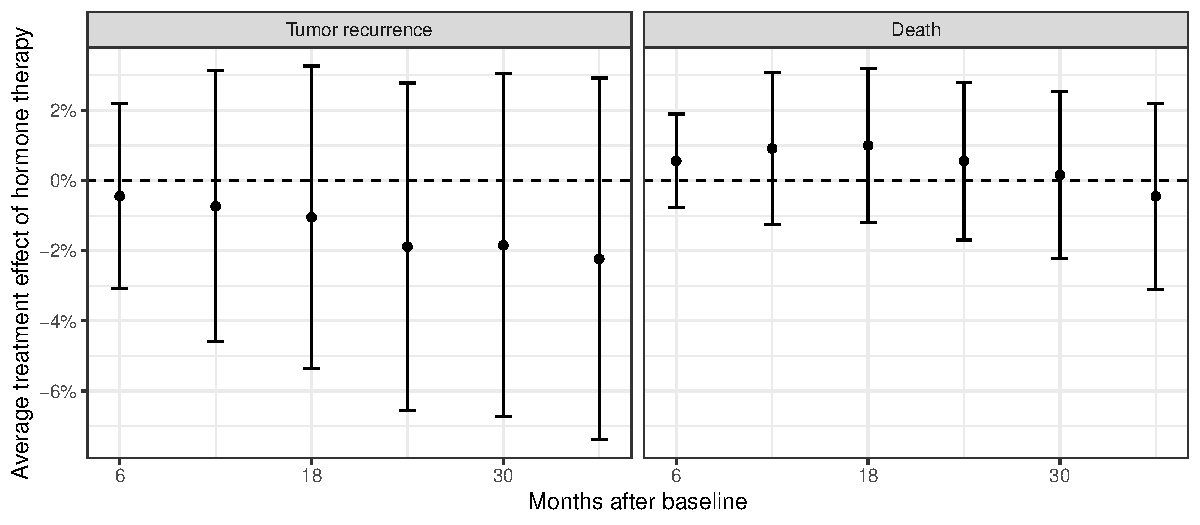
\includegraphics[width=1\linewidth]{./zelefsky-data-target-par.pdf}}
  \caption[]{Estimates of the average treatment effect of hormone therapy on the
    risk of tumor recurrence and death obtained from the prostate cancer study
    analyzed by \cite{kattan2000pretreatment}. The estimates are based on the
    estimator defined in equation~(\ref{eq:one-step-comp-ate}) with point wise
    95\% confidence intervals calculated as described in
    Section~\ref{sec:targeted-learning}. The estimates of the nuisance
    parameters are provided by the state learner.}
  \label{fig:zelefski-real-target}
\end{figure}



\section{Discussion}
\label{sec:discussion}

We have proposed a new super learner that can be used with right-censored data
and competing events. Compared to existing methods, the advantage of the state
learner is that it does not depend on a pre-specified estimator of the censoring
distribution, but selects one automatically based on the provided library
\( \mathcal{B} \). Furthermore, the state learner neither requires evaluation of
the density of \( \Lambda_j \) nor assumes a particular semi-parametric
structure for $\Lambda_j$. In the remainder of this section we point to some
limitations of our proposal and discuss avenues for further research.

A major advantage of the state learner is that performance of each combination
of learners is measured in terms of observable quantities. This means that no
additional nuisance parameters need to be estimated to evaluate the loss. The
drawback with this approach is that we are rarely interested in features of the
observed data distribution when the data are right-censored. The finite sample
oracle inequality in Corollary~\ref{cor:oracle-prop} concerns the function
\( F \), which is a feature of \( P \in \mathcal{P} \), while what we are
typically interested in is \( \Lambda_j \) or \( S \), which are features of
\( Q \in \mathcal{Q} \). We emphasize that while the state learner provides us
with estimates of \( \Lambda_j \) and $\Gamma$ based on libraries
\( \mathcal{A}_j \) and \( \mathcal{B} \), performance are not assessed directly
for these parameters, but only jointly for estimation of the parameter \( F \).
For settings without a competing risk, our numerical studies suggest that
measuring performance with respect to estimation of \( F \) also leads to good
performance for estimation of \( S \). Further research on this topic, both
numerical and theoretical, is warranted.

% In the context of targeted learning, a drawback of the state learner is that the
% doubly robustness property defined in equation~(\ref{eq:dr-property}) seem to be
% lost because we only use a single nuisance parameter estimator. As defined here,
% however, the state learner is build using libraries for the conditional
% cause-specific cumulative hazard functions, so some doubly robustness might be
% preserved.

Our proposed super learner can be implemented with a broad library of learners
using existing software, for instance the \texttt{R}-package
\texttt{riskRegression} \citep{Gerds_Ohlendorff_Ozenne_2023}. Furthermore, while
the library \( \mathcal{F}(\mathcal{A}_1,\mathcal{A}_2,\mathcal{B}) \) consists
of \( |\mathcal{A}_1||\mathcal{A}_2||\mathcal{B}| \) learners, as long as we
have sufficient memory we need only fit
\( |\mathcal{A}_1| +|\mathcal{A}_2| + |\mathcal{B}| \) learners in each fold. To
evaluate the performance of each learner we need to perform
\( |\mathcal{A}_1||\mathcal{A}_2||\mathcal{B}| \) operations to calculate the
integrated Brier score in each hold-out sample, one for each combination of the
fitted models, but these operations are often negligible compared to fitting the
models. Hence the state learner is essentially no more computationally demanding
than any procedure that uses super learning to learn $\Lambda_1$, $\Lambda_2$,
and $\Gamma$ separately. While our proposal is based on constructing the library
\( \mathcal{F} \) from libraries for learning \( \Lambda_1 \), $\Lambda_2$, and
$\Gamma$, it would also be of interest to consider learners that estimate
\( F \) directly.

In our numerical studies, we only considered learners of $\Lambda_j$ and
$\Gamma$ that provide cumulative hazard functions which are piece-wise constant
in the time argument. This simplifies the calculation of \( F \) as the
integrals in equation~(\ref{eq:transition}) reduce to sums. When $\Lambda_j$ or
\( \Gamma \) are absolutely continuous in the time argument, calculating \( F \)
is more involved, but we expect that a good approximation can be achieved by
discretization. In the future, we intend to investigate the performance of the
state learner when using a broader library of learners in more comprehensive
simulation studies.



\appendix

\section{Theoretical guarantees for the state learner}
\label{sec:proof-proposition}

In this section we provide proofs of the results stated in
Section~\ref{sec:theor-results-prop}.

Define
\( \bar{B}_{\tau,0}(F, o) = \bar{B}_{\tau}(F, o) - \bar{B}_{\tau}(F_0, o) \) and
\( R_{0}(F) = P_0{[\bar{B}_{\tau,0}(F, \blank)]} \).
\begin{lemma}
  \label{lemma:norm}
  \( R_{0}(F) = \Vert F - F_0 \Vert_{P_0}^2 \), where \( \Vert \blank \Vert_{P_0}\) is defined
  in equation~(\ref{eq:norm}).
\end{lemma}
\begin{proof}
  For any \( t \in [0, \tau] \) and \( k\in \{0,1,2\} \) we have
  \begin{align*}
    & \E_{P_0}{\left[ (F(t, k, X) - \1{\{\eta(t) = k \}})^2 \right]}
    \\
    & =    \E_{P_0}{\left[ (F(t, k, X) - F_0(t, k, X) + F_0(t, k, X) - \1{\{\eta(t) = k
      \}})^2 \right]}
    \\
    & =    \E_{P_0}{\left[ (F(t, k, X) - F_0(t, k, X))^2\right]}
      + \E_{P_0}{\left[ (F_0(t, k, X) - \1{\{\eta(t) = k \}})^2\right]}
    \\
    & \quad
      + 2\E_{P_0}{\left[ (F(t, k, X) - F_0(t, k, X))(F_0(t, k, X) - \1{\{\eta(t) = k
      \}})\right]}
    \\
    & =    \E_{P_0}{\left[ (F(t, k, X) - F_0(t, k, X))^2\right]}
      + \E_{P_0}{\left[ (F_0(t, k, X) - \1{\{\eta(t) = k \}})^2\right]},
  \end{align*}
  where the last equality follows from the tower property. Hence, using Fubini,
  we have
  \begin{equation*}
    P{[\bar{B}_{\tau}(F, \blank)]}
    = \Vert F - F_0 \Vert_{P_0}^2 + P_0{[\bar{B}_{\tau}(F_0, \blank)]}.
  \end{equation*}
\end{proof}

\begin{proof}[Proof of Proposition~\ref{prop:stric-prop}]
  The result follows from Lemma~\ref{lemma:norm}.
\end{proof}

In the following, let $\Theta$ denote the function space consisting of all
conditional state occupation probability functions for some measure \( P \) as
defined in equation~(\ref{eq:F-def}).

\begin{proof}[Proof of Corollary~\ref{cor:oracle-prop}]
  First note that minimising the loss \( \bar{B}_{\tau} \) is equivalent to
  minimising the loss \( \bar{B}_{\tau,0} \), so the discrete super learner and
  oracle according to \( \bar{B}_{\tau} \) and \( \bar{B}_{\tau,0} \) are
  identical. By Lemma~\ref{lemma:norm}, \( R_0(F) \geq 0 \) for any
  \( F \in \Theta \), and so using Theorem 2.3 from \citep{vaart2006oracle} with
  \( p=1 \), we have that for all \( \delta >0 \),
\begin{align*}
  \E_{P_0}{\left[ R_0(\hat{\phi}_n(\data_n^{-k})) \right]}
  \leq
  &(1+2\delta)\E_{P_0}{\left[ R_0(\tilde{\phi}_n(\data_n^{-k})) \right]}
  \\
  & \quad + (1+\delta) \frac{16 K}{n}
    \log(1 + |\mathcal{F}_n|)\sup_{F \in \Theta}
    \left\{
    M(F) + \frac{v(F)}{R_0(F)}
    \left(
    \frac{1}{\delta} + 1
    \right)
    \right\}
\end{align*}
where for each \( F \in \Theta \), \( (M(F), v(F)) \) is some Bernstein pair for
the function \(o \mapsto \bar{B}_{\tau,0}(F, o) \). As
\( \bar{B}_{\tau,0}(F, \blank) \) is uniformly bounded by \( \tau \) for any
\( F \in \Theta \), it follows from section 8.1 in \citep{vaart2006oracle} that
\( (\tau, 1.5 P_0{[\bar{B}_{\tau,0}(F, \blank)^2]}) \) is a Bernstein pair for
\( \bar{B}_{\tau,0}(F, \blank) \). Now, for any \( a,b,c \in \R \) we have
\begin{align*}
  (a-c)^2 - (b-c)^2
  & = (a-b+b-c)^2 - (b-c)^2
  \\
  & = (a-b)^2 + (b-c)^2 +2(b-c)(a-b) - (b-c)^2
  \\
  & = (a-b)
    \left\{
    (a-b) +  2(b-c)
    \right\}
  \\
  & = (a-b)
    \left\{
     a + b -2c
    \right\},
\end{align*}
so using this with \( a=F(t, k, x) \), \( b=F_0(t, k, x) \), and
\( c = \1{\{\eta(t) = k\}} \), we have by Jensen's inequality
\begin{align*}
  & P_0{[\bar{B}_{\tau,0}(F, \blank)^2]}
  \\
  & \leq
    2\tau\E_{P_0}{\left[
    \sum_{k=0}^{3} \int_0^{\tau}
    \left\{
    \left(
    F(t, k, X) - \1{\{\eta(t) = k\}}
    \right)^2
    -
    \left(
    F_0(t, k, X) - \1{\{\eta(t) = k\}}
    \right)^2
    \right\}^2
    \diff t 
    \right]}
  \\
  & =2\tau
    \E_{P_0}\Bigg[
    \sum_{k=0}^{3} \int_0^{\tau}
    \left(
    F(t, k, X) - F_0(t, k, X)
    \right)^2
  \\
  & \quad \quad \quad\quad \quad \quad \times
    \left\{
    F(t, k, X) +  F_0(t, k, X)-2 \1{\{\eta(t) = k\}}
    \right\}^2
    \diff t 
    \Bigg]
  \\
  & \leq
    8\tau \E_{P_0}{\left[
    \sum_{k=0}^{3} \int_0^{\tau}
    \left(
    F(t, k, X) - F_0(t, k, X)
    \right)^2
    \diff t 
    \right]}.
  \\
  & =
    8\tau \Vert F - F_0 \Vert_{P_0}^2.
\end{align*}
Thus when \( v(F) = 1.5 P_0{[\bar{B}_{\tau,0}(F, \blank)^2]} \) we have by
Lemma~\ref{lemma:norm}
\begin{equation*}
  \frac{v(F)}{R_0(F)}
  = 1.5 \frac{P_0{[\bar{B}_{\tau,0}(F, \blank)^2]}}{P_0{[\bar{B}_{\tau,0}(F, \blank)]}}
  \leq 12 \tau,
\end{equation*}
and so using the Bernstein pairs \( (\tau, 1.5 P_0{[\bar{B}_{\tau,0}(F, \blank)^2]}) \) we have
\begin{equation*}
  \sup_{F \in \Theta}
  \left\{
    M(F) + \frac{v(F)}{R_0(F)}
    \left(
      \frac{1}{\delta} + 1
    \right)
  \right\}
  \leq \tau
  \left(
    13 + \frac{12}{\delta}
  \right),
\end{equation*}
For all $\delta>0$ we thus have
\begin{align*}
  \E_{P_0}{\left[ R_0(\hat{\phi}_n(\data_n^{-k})) \right]}
  \leq
  &(1+2\delta)\E_{P_0}{\left[ R_0(\tilde{\phi}_n(\data_n^{-k})) \right]}
  \\
  & \quad
    + (1+\delta)\log(1 + |\mathcal{F}_n|) \tau \frac{16 K}{n}
    \left(
    13 + \frac{12}{\delta}
    \right),
\end{align*}
and then the final result follows from Lemma~\ref{lemma:norm}.
\end{proof}

\begin{proof}[Proof of Corollary~\ref{cor:asymp-cons}]
  By definition of the oracle and Lemma~\ref{lemma:norm},
  \( \E_{P_0}{\left[ \Vert \tilde{\phi}_n(\data_n^{-k}) - F_0 \Vert_{P_0}^2 \right]}
  \leq \E_{P_0}{\left[ \Vert \phi_n(\data_n^{-k}) - F_0 \Vert_{P_0}^2 \right]} \) for
  all \( n \in \N \). The results then follows from
  Corollary~\ref{cor:oracle-prop}.
\end{proof}


\section{The state learner with targeted learning}
\label{sec:state-learner-with}

In this section show that a product structure is preserved when the estimator
$\bar\Psi(\hat{F}_n, \hat{H}_n)$ is used instead of
$\tilde\Psi(\hat{\Lambda}_n, \hat{\Gamma}_n, \hat{H}_n)$.


\begin{proof}[Proof of Proposition~\ref{prop:dr-structure}]
  For notational convenience we suppress \( X \) in the following. The final
  result can be obtained by adding the argument \( X \) to all functions and
  averaging. We use the relations from equation~(\ref{eq:7}) to write
  \begin{align*}
    & \int_0^{\tau} w(s) 
      \left\{
      \Gamma(s) - \hat{\Gamma}_n(s)
      \right\}
      [\Lambda - \hat{\Lambda}_n](\diff s)
    \\
    & =
      \int_0^{\tau} w(s) 
      \left\{
      \int_0^s \frac{F(\diff u, 2)}{F(u-, 0)} -
      \int_0^s \frac{\hat{F}_n(\diff u, 2)}{\hat{F}_n(u-, 0)}  -
      \right\}
      \left[
      \frac{F(\diff s, 1)}{F(s-, 0)}
      - \frac{\hat{F}_n(\diff s, 1)}{\hat{F}_n(s-, 0)}
      \right]
    \\
    & =
      \int_0^{\tau} w(s) 
      \Bigg\{
      \int_0^s 
      \left(
      \frac{1}{F(u-, 0)} -  \frac{1}{\hat{F}_n(u-, 0)}
      \right) F(\diff u, 2)
    \\
    & \qquad\qquad \qquad
      +
      \int_0^s \frac{1}{\hat{F}_n(u-, 0)} 
      \left[
      F(\diff u, 2) - \hat{F}_n(\diff u, 2)
      \right]
      \Bigg\}
    \\
    & \qquad\qquad \times
      \left[
      \left(
      \frac{1}{F(s-, 0)} -
      \frac{1}{\hat{F}_n(s-, 0)}
      \right)F(\diff s, 1)
       + \frac{1}{\hat{F}_n(s-, 0)}
      \left(
      F(\diff s, 1) -
      \hat{F}_n(\diff s, 1)
      \right)
      \right]
    \\
    &
      = \int_0^{\tau} 
      \int_0^s
      w(s) 
      \left(
      \frac{1}{F(u-, 0)} -  \frac{1}{\hat{F}_n(u-, 0)}
      \right) 
      \left(
      \frac{1}{F(s-, 0)} -
      \frac{1}{\hat{F}_n(s-, 0)}
      \right)F(\diff u, 2)F(\diff s, 1)
    \\
    & \quad +
      \int_0^{\tau}
      \int_0^s
      w(s) 
      \left(
      \frac{1}{F(u-, 0)} -  \frac{1}{\hat{F}_n(u-, 0)}
      \right) \frac{F(\diff u, 2) }{\hat{F}_n(u-,0)}
      \left(
      F(\diff s, 1) -
      \hat{F}_n(\diff s, 1)
      \right)
    \\
    & \quad +
      \int_0^{\tau} 
      \int_0^s      
      \frac{w(s) }{\hat{F}_n(u-, 0)} 
      \left[
      F(\diff u, 2) - \hat{F}_n(\diff u, 2)
      \right]
      \left(
      \frac{1}{F(s-, 0)} -
      \frac{1}{\hat{F}_n(s-, 0)}
      \right)F(\diff s, 1)
    \\
    & \quad +
      \int_0^{\tau} 
      \int_0^s      
      \frac{w(s) }{\hat{F}_n(u-, 0)} 
      \left[
      F(\diff u, 2) - \hat{F}_n(\diff u, 2)
      \right]
      \frac{1}{\hat{F}_n(s-, 0)}
      \left(
      F(\diff s, 1) -
      \hat{F}_n(\diff s, 1)
      \right).
  \end{align*}
  Consider the first term on the right hand side. Defining
  \begin{equation*}
    w_n^*(t)  = 
    \left(
      F(t-, 0)
      - \hat{F}_n(t-, 0)
    \right)
    \left(
      \frac{1}{F(t-, 0)}
      - \frac{1}{\hat{F}_n(t-, 0)}
    \right),
  \end{equation*}
  we can write
  \begin{align*}
    & \int_0^{\tau} 
      \int_0^s
      w(s) 
      \left(
      \frac{1}{F(u-, 0)} -  \frac{1}{\hat{F}_n(u-, 0)}
      \right)      
      \left(
      \frac{1}{F(s-, 0)} -
      \frac{1}{\hat{F}_n(s-, 0)}
      \right)F(\diff u, 2)F(\diff s, 1)
    \\
    & =
      \int_0^{\tau} 
      \int_0^s
      w(s)
      w_n^*(u) 
      \left(
      F(u-, 0) - \hat{F}_n(u-, 0)
      \right)
    \\
    & \qquad \qquad \quad
      \times
      w_n^*(s) 
      \left(
      F(s-, 0) - \hat{F}_n(s-, 0)
      \right)       
      F(\diff u, 2)F(\diff s, 1)
    \\
    & =
      \int_0^{\tau} 
      \int_0^s
      w_n^a(s,u)
      \left(
      F(u-, 0) - \hat{F}_n(u-, 0)
      \right)
      \left(
      F(s-, 0) - \hat{F}_n(s-, 0)
      \right)       
      F(\diff u, 2)F(\diff s, 1),
  \end{align*}
  where we have defined \( w_n^a(s,u) = w(s)w^*_n(s)w^*_n(u) \). By assumption,
  \( w_n^a(s,u) \) is uniformly bounded. The same approach can be applied to the
  three remaining terms which gives the result.
\end{proof}

\bibliography{bib.bib}

\end{document}